\chapter{Cammini Minimi in un Grafo}
Il problema dei cammini minimi su grafi è uno dei problemi più importanti e studiati al mondo e trova importanti applicazioni in vari campi come le reti di telecomunicazioni ecc.

Richiamiamo alcune definizioni:
\begin{itemize}
    \item Sia $V$ un insieme di nodi
    \item Sia $E \subset V \times V: (v,v) \notin E:\forall v \in V$.
    \item La coppia $G=(V,E)$ è un grafo orientato con $V$ l'insieme dei nodi ed $E$ l'insieme degli archi. 
    \item Sia $w:E\rightarrow R$ una funzione peso o costo, $(G,w)$ si dice grafo pesato.
\end{itemize}

Dato $G=(V,E)$ con $V=\{1,\dots,n\}$ la \textbf{matrice di adiacenza} associata al grafo è la matrice $A$ di dimensione $n \times n$ tale che $A_{ij}$ è 1 se $(i,j)\in E$ o 0 altrimenti. 

Dato $G=(V,E)$ le \textbf{liste di adiacenze} associate al grafo sono gli insieme $Adj_g(u) = \{v \in V: (u,v)\in E\}$.

Sia $G=(V,E)$  un grafo con una funzione peso $w:E \rightarrow R$, siano $u,v \in V$ si dice \textbf{cammino da $u$ a $v$} è una sequenza $\pi = (v_0, \dots, v_k)$ di nodi contigui di G tale che:
\begin{itemize}
    \item $v_0 = u, v_k = v$.
    \item $(v_{i-1},v_i)\in E$ per $i=1, \dots, k$
\end{itemize} 
Poniamo $w(\pi) = \sum_{k}^{i=1}w(v{i-1},v_i)$  con k la lunghezza del cammino, $v_0$ la testa e $v_k$ la coda.

Siano $\pi_1 = (v_0, \dots, v_k)$ e $\pi_2 = (v_k, \dots, v_l)$ due cammini, scriviamo $\pi_1;\pi_2$ per indicare la \textbf{concatenazione di $\pi_1$ e $\pi_2$} cioè il cammino che è la somma dei due cammini sia in termini di percorso che in termini di peso. 

Poniamo $\delta(u,v)= \min\{w(\pi): \pi \in path(G,u,v)\}$. Sia un cammino $\pi \in paths(G;u,v)$ è \textbf{minimo} se $w(\pi) = \delta(u,v)$. 
Da questo possiamo definire vari problemi:
\begin{enumerate}
    \item Dato un grafo pesato calcolare $\delta(u,v)$.
    \item Dato un grafo pesato e dato un vertice appartenente al grafo detto \textbf{sorgente}, calcolare $\delta(s,v)$ per ogni $v \in V$.
    \item Dato un grafo pesato e dato un vertice detto \textbf{destinazione}, calcolare $\delta(v,t)$ per ogni $v \in V$.
    \item Dato un grafo pesato calcolare $\delta(u,v)$ per ogni vertice $u,v \in V$. 
\end{enumerate}

Un grafo \textbf{ammette cammini minimi da s} se $\delta(s,u)\neq - \inf$ per ogni vertice $v \in V$
Un grafo \textbf{ammette cammini minimi} se $\delta(u,v)\neq - \inf$ per ogni vertice $u,v \in V$. 

Diciamo che un grafo ammette cammini minimi se e solo se ammette cammini minimi da ciascuno dei suoi nodi. 

Una condizione necessaria e sufficiente perché un grafo pesato ammetta cammini minimi da una sorgente s è che \textbf{non vi sia alcun ciclo di peso negativo raggiungibile da s}.

Condizione necessaria e sufficiente perché un \textbf{grafo ammetta cammini minimi} è che non contenga archi di peso negativo. Segue che se la funzione peso non è negativa allora ammette sempre cammini minimi. Allo stesso modo se un grafo è aciclico ammette sempre cammini minimi. 

Sia $\pi=(v_0,\dots, v_k)$ un cammino minimo in $G=(V,E)$ e $w:E\rightarrow R$, allora il \textbf{sottocammino} $\pi_{ij}=v_i,\dots, v_j$ per ogni $0\leq i \leq j \leq k$ è minimo. Si può dimostrare banalmente perché se esistesse un altro cammino minimo da i a j, allora quello di partenza non sarebbe più minimo.

Per cercare di memorizzare tutti i cammini minimi a singola sorgente (anziché andare a memorizzare tutto in delle liste), possiamo utilizzare \textbf{un grafo dei cammini minimi} che non è altro che un grafo composto da tutti gli archi che compongono i cammini da s a tutti i vertici.

Sia $min\_paths(G;s)\neq 0$ allora $paths(G'_s;s)=min\_paths(G;s)$ Dobbiamo dimostrare la doppia inclusione:
\begin{itemize}
    \item CASO $min\_paths \subseteq paths$: Dalla definizione di $G'_s$ segue immediatamente che $\text{MIN\_PATHS} \subseteq \text{PATHS}$.
    \item CASO $paths(G'_s;s) \subseteq min\_paths$ Immaginiamo che esista almeno un percorso $\pi$ dentro $G'_s$ che però NON è un cammino minimo nel grafo originale ($\pi \notin \text{MIN\_PATHS}(G; s)$). Tra tutti questi ipotetici percorsi "sbagliati", prendiamo quello con il \textbf{minor numero di archi}.
    Poiché $\pi$ è il "primo" percorso sbagliato se togliamo l'ultimo pezzo, quello che rimane deve essere giusto. Quindi il peso di questo pezzo è esattamente la distanza minima: $w(\pi') = \delta(s, v_{k-1})$. Il peso di tutto il percorso $\pi$ è la somma del prefisso ottimo + l'ultimo arco:
    \[w(\pi) = w(\pi') + w(v_{k-1}, v_k) = \delta(s, v_{k-1}) + w(v_{k-1}, v_k)\]
    Consideriamo un vero cammino $\bar{\pi}$ che passa per quell'ultimo arco, sappiamo che per le proprietà dei cammini minimi la distanza vera per arrivare a $v_k$, cioè $\delta(s, v_k)$, è uguale alla distanza per arrivare a $v_{k-1}$ più il peso dell'arco:
    \[\delta(s, v_k) = \delta(s, v_{k-1}) + w(v_{k-1}, v_k)\]
    Ma qui arriviamo a un assurdo poiché abbiamo che $w(\pi) = \delta(s, v_{k-1}) + w(v_{k-1}, v_k)$ e che $\delta(s, v_k) = \delta(s, v_{k-1}) + w(v_{k-1}, v_k)$.che dimostra che $w(\pi) = \delta(s, v_k)$ che contraddice l'ipotesi che $\pi$ non è minimo.
\end{itemize}

Sia $(G,w)$ un grafo pesato e sia $s\in V$ una sorgente. Supponiamo che il grafo ammetta cammini minimi da $s$, allora esiste un \textbf{albero di cammini minimi} $G''_s=(V'',E''_s):V''\subseteq V, E''_s \subseteq E$ radicato in s contenente esattamente un cammino minimo da s in ciascun nodo raggiungibile da esso. Per costruirlo, ci basta fare una visita BFS o DFS da s nel grafo dei cammini minimi. Per rappresentare in maniera efficiente questo albero, utilizziamo la funzione $pred$ per cui ogni nodo ha un riferimento al precedente verso la radice.
\begin{figure}[H]
    \centering
    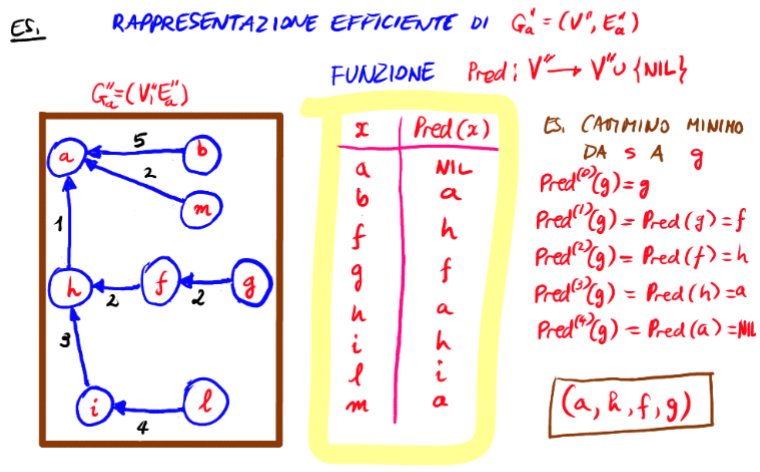
\includegraphics[width=0.5\linewidth]{Images/cammini_minimi/rappresentazione_efficiente.png}
\end{figure}

Dato un grafo non orientato $G=(V,E)$ con funzione peso $w:E \rightarrow R$ e sorgente $s\in V$, \textbf{non è necessariamente vero che tra i suoi alberi di cammini minimi da s ci debba essere un mst}.
\begin{figure}[H]
    \centering
    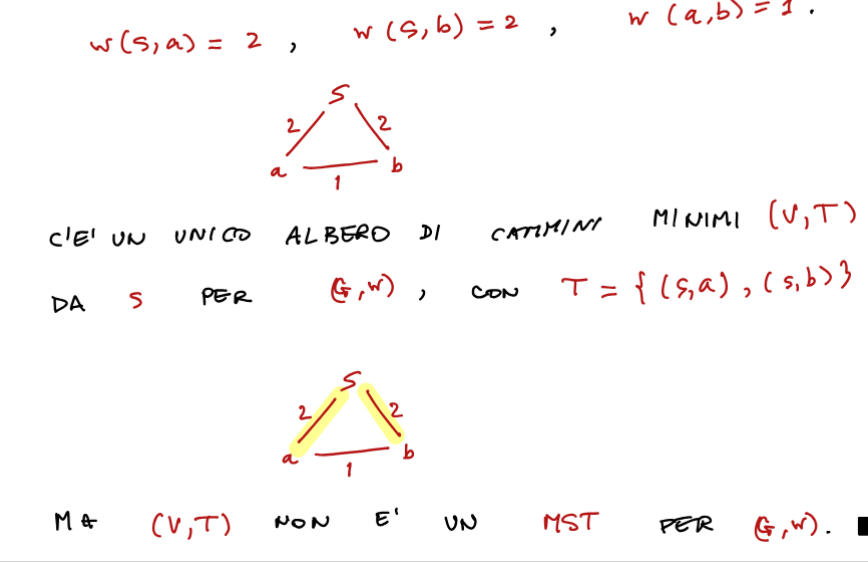
\includegraphics[width=0.6\linewidth]{Images/cammini_minimi/mst_cammini_minimi.png}
\end{figure}


\section{Algoritmi per Cammini Minimi da Una Sorgente}
Descriveremo algoritmi basati su \textbf{tecniche di Label Correctin/Setting}. In pratica, dato un grafo $G=(V,E)$ con funzione peso $w:E \rightarrow R$ e sorgente $s\in V$, viene mantenuta una funzione $d:V \rightarrow R \cup \{\inf\}$ che sarà la nostra \textbf{stima della distanza} e faremo in modo tale che valga sempre che $d \geq \delta_{G_s}$ e che alla fine della computazione valga $d=\delta_{G_s}$.

Possiamo iniziare a impostare le distanze come segue:
\begin{align*}
    &d[s]= 0;\\
    &d[v]= \inf; \forall v \in V/\{s\}
\end{align*}
L'albero dei cammini minimi sarà rappresentato da un array di predecessori costruito insieme al calcolo della distanza $\delta_{G_s}$. Per farlo, basterà inizialmente porre il predecessore di ogni nodo a $null$.
\begin{figure}[H]
    \centering
    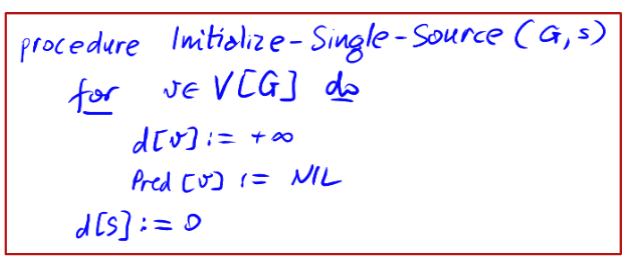
\includegraphics[width=0.6\linewidth]{Images/cammini_minimi/initialize_ss.png}
\end{figure}
Per aggiornare queste due funzioni, utilizzeremo la così detta procedura di \textbf{Relax} che sarà alla base di molti algoritmi che vedremo. In pratica, se la distanza $d[v]$ è maggiore rispetto alla distanza $d[u]+w(u,v)$, allora abbiamo trovato un cammino migliore che va dalla sorgente a v che passa prima da u.
\begin{figure}[H]
    \centering
    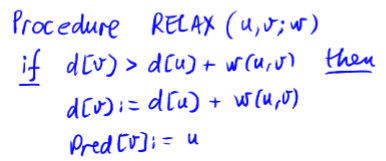
\includegraphics[width=0.4\linewidth]{Images/cammini_minimi/relax.png}
\end{figure}
Da questo, segue l'algoritmo \textbf{Generic Single-Source Shortest-Path (GSSSP)}:
\begin{figure}[H]
    \centering
    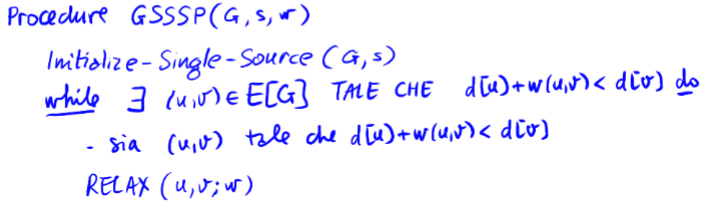
\includegraphics[width=0.6\linewidth]{Images/cammini_minimi/gsssp.png}
\end{figure}
Durante l'esecuzione di GSSSP, varrà che:
\begin{itemize}
    \item La funzione $d$ decrescerà monotomicamente.
    \item Se $d[x] < \inf$, allora esiste un cammino da $s$ a $x$ di peso minore o uguale a $d[x]$.
    \item Vale sempre $\delta_{G_s} \leq d$, cioè, $\delta_{G_s}(x) \leq d[x]$. 
\end{itemize}
Passiamo a dimostrare questi punti:
\begin{itemize}
    \item La prima proprietà segue direttamente per induzione sul numero di esecuzione della procedura relax. A ogni relax, il valore d può solo diminuire.
    \item La seconda si dimostra per induzione:
        \begin{itemize}
            \item \textbf{Caso Base}: Inizialmente abbiamo che $d[x] < \inf$ solo per $x=s$ e, in particolare $d[s]=0$.
            \item \textbf{Passo induttivo}: Sia x un nodo in G tale che $d[x] < \inf$ dopo una certa relax. Indicheremo $d^{-}$ e $d^{+}$ il valore della funzione d immediatamente prima e immediatamente dopo. Abbiamo anche qui due casi:
            \begin{itemize}
                \item \textbf{Caso 1:} $d^{-}[x] = d^{+}$ cioè non cambia niente, poiché $d^{-}[x] < \inf$, per ipotesi induttiva esiste un cammino da $s$ a $x$ di peso $w(\pi_{sx}) \leq d^{-}[x]$.
                \item \textbf{Caso 2:} $d^{+}[x]<d^{-}[x]$ allora in questo caso avremo che $d^+[x] = d^-[u] + w(u, x)\leq \inf$. Per ipotesi induttiva, esiste un cammino reale $\pi_{su}$ che va dalla sorgente $s$ fino a $u$ e il suo peso è $w(\pi_{su}) \le d^-[u]$. Creiamo un nuovo cammino $\pi_{sx}$ semplicemente "incollando" l'arco $(u, x)$ alla fine del cammino $\pi_{su}$ e questo, avrà peso:
                \[w(\pi_{sx}) = w(\pi_{su})+ w(u,x) \leq d^-[u] + w(u,x) = d^+[x]\]
            \end{itemize}
        \end{itemize}
    \item Anche il terzo punto si può dimostrare per induzione:
        \begin{itemize}
            \item \textbf{Caso Base}: Anche in questo caso, poiché $\delta_{G_s}(s) \leq 0$ e per ogni $x \in V$ vale che $\delta_{G_s}(x) \leq \inf = d[x]$, allora prima della procedura relax vale che $\delta_{G_s} \leq d$.
            \item \textbf{Passo Induttivo}: Supponiamo che valga $\delta_{G_s} \leq d$ poco prima di relax $(u,v;w)$, sia $d^-$ e $d^+$ come prima. Per ipotesi induttiva $\delta_{G_s} \leq d^-$ e $d^+[x] = d^-[x] \forall x \neq v$. Per il punto due esiste, esiste un cammino $\pi_{sx}$ tale che $w(\pi_{sx}) \leq d^+[x]$ e, dunque, $\delta_{G_s}(x)\leq w(\pi_sx) \leq d^+[x]$. Quindi vale quanto detto. 
        \end{itemize}
\end{itemize}

\textbf{Lemma:}\\
Sia $(G,w)$ tale che $G=(V,E)$ e $w:E\rightarrow R$ e sia $s \in V$. Sia $f:V\rightarrow R \cup \{\inf\}$ tale che $f \geq \delta_{G_s}$ e $f(s)\leq 0$, allora le seguenti condizioni sono equivalenti:
\begin{itemize}
    \item (a): $(\forall(u,v) \in E), \quad f(v) \leq f(u)+ w(u,v)$. \footnote{Per ogni arco del grafo, la stima per arrivare a $v$ è già migliore (o uguale) di quella che otterremmo passando per $u$}
    \item (b): $f=\delta_{G_s}$.\footnote{La nostra funzione $f$ coincide esattamente con le distanze minime vere. Abbiamo trovato la soluzione perfetta.}
\end{itemize}
Dimostriamolo:\\
\begin{enumerate}
    \item \textbf{Ipotesi per assurdo} \\
    Supponiamo per assurdo che valga la prima proprietà (a) ma che $f \neq \delta_{G_s}$. 
    
    \item \textbf{Definizione dell'insieme $P_d$} \\
    Consideriamo l'insieme dei cammini in cui la stima è incoerente (stima maggiore del peso reale):
    \[P_d = \{ \pi \in \text{paths}(G;s) : f(\text{tail}(\pi)) > w(\pi) \}\]
    Osserviamo che la sorgente $s$ non appartiene all'insieme ($s \notin P_d$), infatti:
    \[f(\text{tail}(s)) = f(s) \leq 0 = w(s)\]
    Poiché $f \neq \delta_{G_s}$ (e sapendo che vale sempre $f \geq \delta_{G_s}$), esiste almeno un nodo $v$ tale che $f(v) > \delta_{G_s}(v)$. Dunque esiste un cammino $\pi_{sv}$ tale che $w(\pi_{sv}) < f(v)$, il che implica che $\pi_{sv} \in P_d$. L'insieme non è vuoto.

    \item \textbf{Scelta del cammino minimo} \\
    Sia $\bar{\pi} \in P_d$ un cammino di \textbf{lunghezza minima}. Sia $k = \text{length}(\bar{\pi})$. \\
    Poiché $s \notin P_d$, deve valere $k \geq 1$. \\
    Sia $\bar{\pi} = (v_0, \dots, v_k)$ con $v_0=s$. Poiché $\bar{\pi} \in P_d$, vale che:
    \[f(v_k) = f(\text{tail}(\bar{\pi})) > w(\bar{\pi})\]

    \item \textbf{Analisi del prefisso} \\
    Consideriamo il cammino $\bar{\pi}'$ che coincide con $\bar{\pi}$ privato dell'ultimo arco $(v_{k-1}, v_k)$. \\
    Per la \textbf{minimalità} di $\bar{\pi}$, si ha che $\bar{\pi}' \notin P_d$. Quindi la stima sul penultimo nodo è corretta:

    \[f(v_{k-1}) = f(\text{tail}(\bar{\pi}')) \leq w(\bar{\pi}')\]

    \item \textbf{Contraddizione} \\
    Mettendo insieme le relazioni ottenute:
    \begin{align*}
        f(v_k) &> w(\bar{\pi}) && (\text{poiché } \bar{\pi} \in P_d) \\
               &= w(\bar{\pi}') + w(v_{k-1}, v_k) && (\text{scomposizione del peso}) \\
               &\geq f(v_{k-1}) + w(v_{k-1}, v_k) && (\text{poiché } \bar{\pi}' \notin P_d)
    \end{align*}
    Otteniamo quindi la disuguaglianza stretta:
    \[f(v_k) > f(v_{k-1}) + w(v_{k-1}, v_k)\]
    Ciò contraddice l'ipotesi iniziale (a) secondo cui $f(v) \leq f(u) + w(u,v)$ deve valere per ogni arco del grafo.
\end{enumerate}
Dimostriamo adesso il viceversa.
\begin{enumerate}
    \item \textbf{Ipotesi e Assurdo} \\
    Supponiamo che valga (b), ovvero che $f = \delta_{G_s}$. \\
    Supponiamo per assurdo che non valga (a), cioè che esista un arco $(u, v) \in E$ tale che:
    \[f(v) > f(u) + w(u, v)\]

    \item \textbf{Esistenza del cammino ottimo verso $u$} \\
    Poiché $-\infty < \delta_{G_s}(u) = f(u) < +\infty$, esiste sicuramente un cammino minimo $\pi_{su}$ da $s$ a $u$ tale che:
    \[w(\pi_{su}) = \delta_{G_s}(u)\]

    \item \textbf{Costruzione del cammino verso $v$} \\
    Consideriamo il cammino $\pi_{sv}$ ottenuto concatenando $\pi_{su}$ con l'arco $(u, v)$:
    \[\pi_{sv} = \pi_{su} ; (u, v)\]
    Il peso di questo cammino è:
    \[w(\pi_{sv}) = w(\pi_{su}) + w(u, v)\]
    \item \textbf{Contraddizione} \\
    Riprendiamo la disuguaglianza dell'ipotesi assurda e sostituiamo i valori:
    \begin{align*}
        f(v) &> f(u) + w(u, v) && (\text{Ipotesi assurda}) \\
        \delta_{G_s}(v) &> \delta_{G_s}(u) + w(u, v) && (\text{Poiché } f = \delta_{G_s}) \\
        \delta_{G_s}(v) &> w(\pi_{su}) + w(u, v) && (\text{Sostituzione peso cammino}) \\
        \delta_{G_s}(v) &> w(\pi_{sv}) && (\text{Definizione di } \pi_{sv})
    \end{align*}

    Abbiamo ottenuto che $\delta_{G_s}(v) > w(\pi_{sv})$. \\
    Questo è \textbf{assurdo}, perché per definizione $\delta_{G_s}(v)$ è il peso del cammino minimo da $s$ a $v$, e non può essere strettamente maggiore del peso di un altro cammino esistente ($\pi_{sv}$).
    
    Pertanto, l'ipotesi assurda cade e deve valere:
    \[(\forall (u,v) \in E) \quad f(v) \leq f(u) + w(u,v)\]
\end{enumerate}
\textbf{Lemma}:\\
Da quanto detto prima, una condizione necessaria e sufficiente perché l'algoritmo GSSSP termini è che $d=\delta_{G_s}$. Banalmente se GSSSP si ferma vale che $d[v] \leq d[u] + w(u,v)$ per tutti i nodi e, per il lemma precedente, $d = \delta_{G_s}$. Allo stesso modo si può dimostra poiché se vale che $d=\delta_{G_s}$ allora per il lemma precedente si ha $d[v] \leq d[u] + w(u,v)$, dunque termina GSSSP.

\textbf{Teorema}:\\
Supponiamo che $(G,w)$ ammetta cammini minimi\footnote{Cioè che non vi siano cicli di peso negativo} da una sorgente s. Siano $d:V \rightarrow R \cup \{\inf\}$ e $pred:V \rightarrow V\cup \{null\}$ le funzioni calcolate dopo una sequenza di relax. Definiamo:
\begin{itemize}
    \item $V_T$: Sono i nodi che abbiamo raggiunto finora.
    \item $E_T$: Sono gli archi che collegano ogni nodo al suo padre.
\end{itemize}
Allora le seguenti proprietà valgono prima e dopo l'esecuzione di $relax(u,v;w)$:
\begin{enumerate}
    \item \textbf{$T$ è un albero radicato in $s$}: Significa che seguendo i padri si arriva sempre alla sorgente $s$, senza girare in tondo.
    \item \textbf{Coerenza delle distanze}: Se cammino dentro questo albero da un nodo $x$ a un nodo $y$, la stima $d[y]$ è sempre maggiore o uguale alla stima $d[x]$ più il peso del cammino da $x$ a $y$.
\end{enumerate}
Dimostriamolo indicando con $d', pred'$ il nuovo valore della funzione $d$ e $pred$ dopo la relax. 
\begin{enumerate}
    \item Se la relax non fa nulla, cioè $d'= d \quad pred' = pred$, allora il teorema è banalmente dimostrato. Se invece abbiamo che:
        \begin{itemize}
            \item $d'[v] = d[u]+w(u,v)$ e $d'[z]=d[z]$ per tutti gli altri nodi.
            \item $pred'[v] = u$ e $pred'[z]=pred[z]$ per tutti gli altri nodi.
        \end{itemize}
    Il rischio è che $T'$ non sia più un albero radicato in s, allora v sarebbe necessariamente su $T_{su}$ e si avrebbe che:
    \begin{align*}
        d[v]+w(T_{vu}) \leq d[u]\\
        d[v] + w(T_{vu}) + w(u,v)\leq d[u]+w(u,v)\\
        w(T_{vu})+w(u,v) \leq d[u] + w(u,v) - d[v] < 0
    \end{align*}
    Cioè $T_{vu};(u,v)$ sarebbe un ciclo di peso negativo e ciò è un assurdo perché altrimenti il problema non ammetterebbe cammini minimi.
    \item Dimostriamo adesso la seconda proprietà, cioè che $d'[x] + w(T'_{xy}) \le d'[y]$. Per farlo, controlliamo le coppie $x,y$ il cui percorso è cambiato e ciò accade solo se il percorso passa per il nuovo arco $(u,v)$.  Immaginiamo di avere la seguente situazione:
    \[x \to \dots \to u \to v \to \dots \to y\]
    Possiamo scomporre il percorso da $x$ a $u$, l'arco $(u,v)$ e il percorso da $v$ a $y$ e vediamo cosa cambia. Notiamo che per $x \to u$ valeva già la vecchia proprietà, cioè $d[x] + w(T_{xu}) \le d[u]$. Per quanto riguarda il nodo v,  abbiamo appena aggiornato il valore: $d'[v] = d[u] + w(u, v)$. Infine, per il pezzo $v \to y$, le distanze relative nell'albero non sono peggiorate.
\end{enumerate}
\textbf{Corollario}:\\
Se l'algoritmo GSSSP termina, allora abbiamo che:
\begin{itemize}
    \item $d = \delta_{Gs}$: I valori numerici calcolati sono esatti.
    \item $T$ è un Albero di Cammini Minimi: L'insieme dei puntatori ai "padri" ($Pred$) forma una struttura ad albero che contiene effettivamente i percorsi più brevi possibili dalla sorgente verso tutti gli altri nodi.
\end{itemize}
Si dimostra banalmente poiché, sia $x$ un nodo raggiungibile da $s$ e sia $T_{sx}$ il cammino nell'albero T da s a x, allora per il lemma precedente abbiamo:
\[\delta_{G_s}(x)\leq w(T_{sx})= d[s] + w(T_{sx}) \leq d[x] = \delta_{G_s}(x)\]
Da cui $w(T_{sx}) = \delta_{G_s}(x)$ cioè il cammino è minimo, dunque T è un albero di cammini minimi. 

\textbf{Lemma}: Se $(G,w)$ ammette cammini minimi, l'esecuzione di GSSSP termina dopo al massimo $\lfloor e (|V[G]|-1)!\rfloor$ passi.

\subsection{GSSSP Ottimizzato}
Se $s \leadsto \dots \leadsto u \to v$ è un cammino minimo da s a v e a un certo punto dell'esecuzione vale che $d[u] = \delta_{G_s}(u)$, allora dopo l'esecuzione della relax dell'arco tra $(u,v)$ per la proprietà di sottostruttura ottima avremo che $d[v] = \delta_{G_s}(v)$. Infatti, dopo la relax avremo che:
\[\delta_{G_s}(v)\leq d[v] \leq d[u]+w(u,v) = w(\pi_{su}+w(u,v))= \delta_{G_s}(v)\]
Da cui segue che $d[v] = \delta_{G_s}(v)$. Dunque se riusciamo ad accertarci che $d[u] = \delta_{G_s}(u)$ per qualche nodo, converrà chiamare la relax su ogni nodo adiacente. Introduciamo quindi il seguente algoritmo:
\begin{figure}[H]
    \centering
    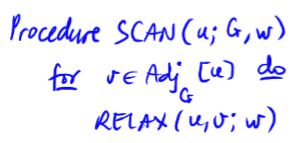
\includegraphics[width=0.3\linewidth]{Images/cammini_minimi/procedure_scan.png}
\end{figure}

Da cui segue la versione ottimizzata di GSSSP che chiameremo OGSSSP:
\begin{figure}[H]
    \centering
    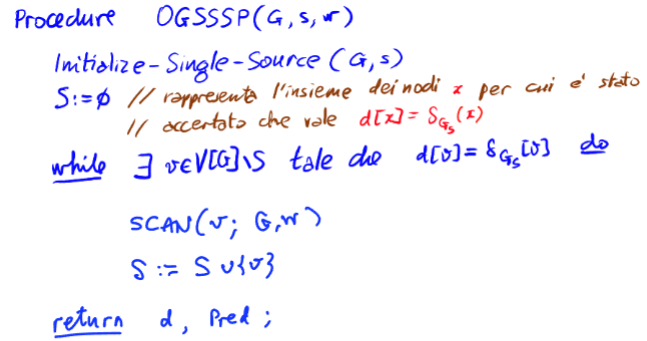
\includegraphics[width=0.6\linewidth]{Images/cammini_minimi/ogsssp.png}
\end{figure}
\textbf{Teorema}\\
Se ci sono ancora \textbf{nodi da visitare} ($V \setminus S \neq \emptyset$), allora esiste sicuramente un nodo $v$ tra questi per cui \textbf{la stima attuale è perfetta}: $d[v] = \delta_{Gs}(v)$.\\
\textbf{Dimostriamolo:}\\
Prendiamo un qualsiasi $u$ non ancora visitato e immaginiamo un cammino minimo che vada dalla sorgente a u: $\pi = (u_0, u_1, \dots, u_k)$. Dato che $s$ è stato visitato (è in $S$) e $u$ no, seguendo questi archi arriveremo a un nodo che non è in $S$ e questo lo indicheremo come $u_{i_0}$. Il predecessore era in S e, dunque era già ottimo, per cui, se rilassiamo l'arco tra $u_{i_0}$ e il suo predecessore, allora anche $u_{i_0}$ sarà ottimo.
La complessità totale di questo algoritmo è $O(V + E) + \text{Tempo per scegliere il nodo giusto}$ cioè il tempo che ci metto a trovare $d[u] = \delta_{G_s}(u)$ e questo dipenderà dagli algoritmi che decidiamo.  

\subsection{Algoritmo di Bellman-Ford}
L'algoritmo di Bellman-Ford non effettua alcun tipo di ottimizzazione nella scelta del "nodo giusto", per cui, quello che fa' è scegliere a ogni iterazione tutti gli archi del grafo e prova a rilassarli. Lo pseudocodice è il seguente:
\begin{figure}[H]
    \centering
    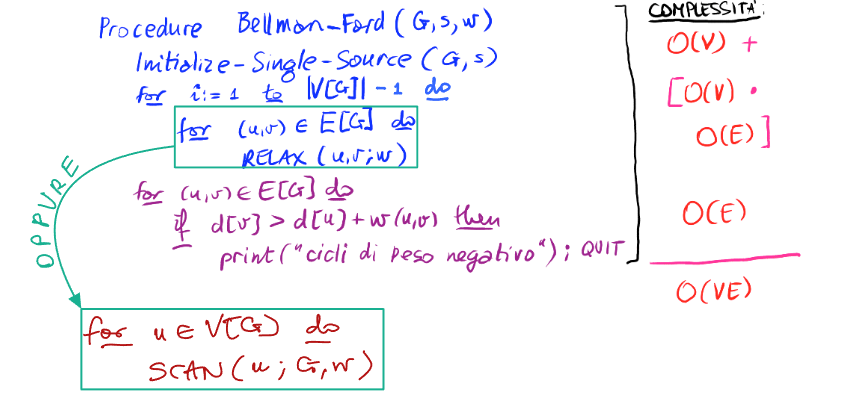
\includegraphics[width=0.7\linewidth]{Images/cammini_minimi/bellman_ford.png}
\end{figure}
Come possiamo vedere, le iterazioni del ciclo sono $|V|-1$ poiché un cammino non può avere più di $|V|-1$ nodi.

Un'altra cosa interessante è che questo algoritmo funziona anche nel caso di archi con cicli di peso negativo poiché se a una prossima iterazione, vi fosse un \textbf{arco che si può ancora rilassare, allora vuol dire che abbiamo archi di peso negativo}, dunque, l'algoritmo Bellman-Ford ce lo segnala.

LA complessità è quindi $O(V)$ per l'inizializzazione, $O(V)*O(E)$ per il ciclo annidato e, infine, $O(E)$ per l'ultimo controllo. In totale la complessità sarà $O(VE)$.

\subsection{Algoritmo di Dijkstra}
Sia $G=(V,E)$ un grafo privo di archi di peso negativo e sia $s \in V$ una sorgente assegnata.
Quello che ci suggerisce di fare l'algoritmo OGSSSP è prendere un nodo per cui $d[v] = \delta_{G_s}(v)$ dai nodi non visitati.  L'algoritmo propone di scegliere il nodo che ha il valore $d[v]$ minimo tra tutti i nodi non visitati. Consideriamo due casi:
\begin{itemize}
    \item \textbf{$s \notin S$}:  All'inizio, l'insieme dei visitati è vuoto. L'unico nodo con distanza finita è la sorgente $s$ ($d[s]=0$) che è il minimo tra i nodi non visitati.
    \item \textbf{Caso $s \in S$, $v \in V \setminus S$ e $d[v] \neq \delta_{G_s}(v)$}:

    In questo caso, poiché la stima non è ottima, allora $\delta_{G_s}(v) < +\infty$ e dunque esiste un cammino minimo reale $\pi_{sv}$ da $s$ a $v$.
    Tale cammino si può scomporre come:
    \[ \pi_{sv} = \pi_{sv'}; (v', v''); \pi_{v''v} \]
    dove l'arco $v' \to v''$ attraversa la frontiera tra l'insieme $S$ e l'insieme $V \setminus S$.

    \begin{figure}[H]
        \centering
        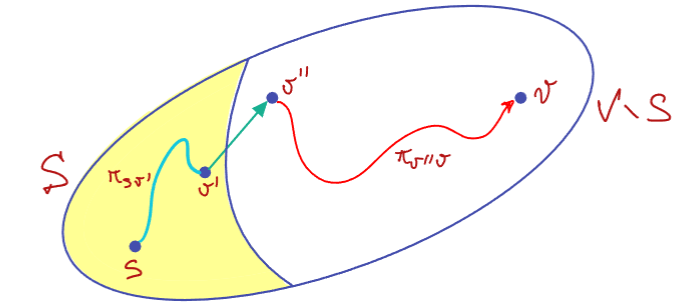
\includegraphics[width=0.6\linewidth]{Images/cammini_minimi/dijkstra_correttezza.png}
    \end{figure}

    Poiché il cammino $\pi_{sv'}; (v', v'')$ è parte di un cammino minimo, vale che $d[v'] = \delta_{G_s}(v')$. Dunque, chiamando $relax(v', v''; w)$, avremo che $d[v''] = \delta_{G_s}(v'')$ per quanto visto precedentemente.
    Seguendo questo ragionamento vediamo che:

    \begin{align*}
        d[v] &> \delta_{G_s}(v) = w(\pi_{sv}) \\
            &= w(\pi_{sv'}; (v', v'')) + w(\pi_{v''v}) \\
            &= \delta_{G_s}(v'') + w(\pi_{v''v}) \\
            &\geq \delta_{G_s}(v'') \quad \text{(poiché } w \ge 0 \text{)} \\
            &= d[v''] \\
            &\geq \min \{ d[u] : u \in V \setminus S \}
    \end{align*}

    Dunque, avremo che:
    \[ d[v] > \min \{ d[u] : u \in V \setminus S \} \]

    E, quindi, possiamo dire che per ogni nodo $\bar{v} \in V \setminus S$ tale che $d[\bar{v}] = \min \{ d[u] : u \in V \setminus S \}$ (ovvero il nodo scelto dall'algoritmo) vale necessariamente che:
    \[ d[\bar{v}] = \delta_{G_s}(\bar{v}) \]
\end{itemize}

Da ciò, segue l'algoritmo di Dijkstra:
\begin{figure}[H]
    \centering
    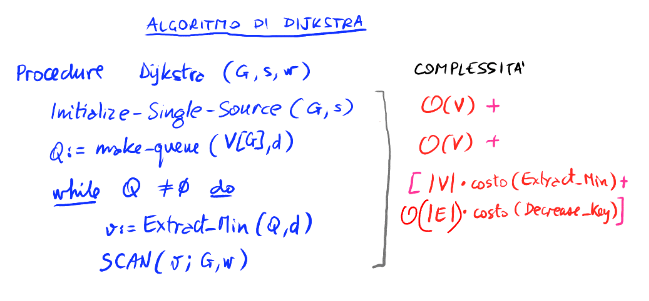
\includegraphics[width=0.6\linewidth]{Images/cammini_minimi/dijkstra_algoritmo.png}
\end{figure}
La complessità dell'algoritmo può dunque variare in base a come implementiamo la coda $Q$:
\begin{figure}[H]
    \centering
    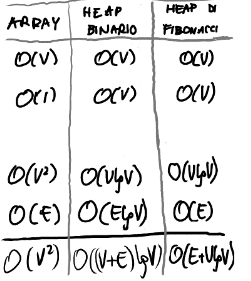
\includegraphics[width=0.2\linewidth]{Images/cammini_minimi/coda_dijkstra.png}
\end{figure}

\subsection{Algoritmo DAG}
Sia $G=(V,E)$ un grafo aciclico on $w:E\to R$ e sia $s \in V$ una sorgente assegnata. Sia $u\in V/S$ tale che $d[u] > \delta_{G_s}(u)$, allora $\delta_{G_s}(u)< \inf$ e dunque esiste un cammino minimo da s a u. \\
Sia $u'$ il predecessore di $u$ in $\pi_{su}$, poiché $d[u] > \delta_{G_s}(u)$, deve valere che $u' \in V/S$,\footnote{Questa cosa deve essere vera poiché se $u'$ fosse stato visitato, allora avremmo già effettuato la relax $u',u$.} pertanto, vale che $u$ ha un predecessore $u' \in V/S$ e, quindi, per ogni nodo $v \in V/S$ i cui predecessori appartengono tutti ad S, vale che $d[v] = \delta_{G_s}(v)$. Cioè \textbf{se ho già visitato tutti i nodi che potrebbero "portare" a $v$ (tutti i suoi potenziali padri), allora la stima di $v$ non può più cambiare}.

Da queste considerazioni, possiamo descrivere questo algoritmo:
\begin{figure}[H]
    \centering
    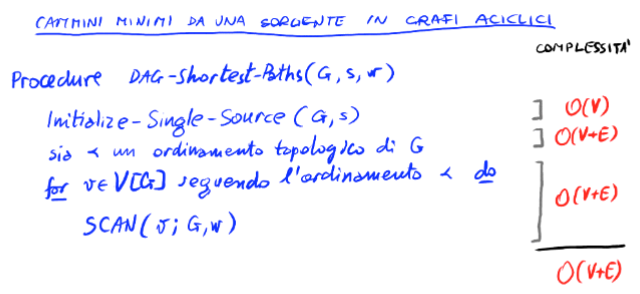
\includegraphics[width=0.7\linewidth]{Images/cammini_minimi/dag.png}
\end{figure}


\section{Cammini Minimi tra Tutte le Coppie}
Da adesso sarà necessario considerare la seguente notazione:
\begin{itemize}
    \item $d[v] \to d[s,v]$ stima della distanza da s a v.
    \item $pred[v] \to pred[s,v]$ predecessore di v in un cammino da s a v.
\end{itemize}

Questo è necessario poiché stiamo passando in un contesto con più sorgenti. Passiamo dunque da un'array a una matrice. Immaginiamo una situazione di questo tipo, siano $v_,1 v_4, v_7$ dei nodi nel grafo come segue:
\begin{figure}[H]
    \centering
    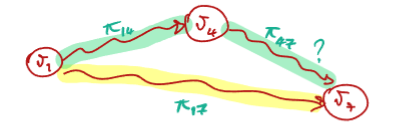
\includegraphics[width=0.4\linewidth]{Images/cammini_minimi/coppie/esempio.png}
\end{figure}
Vediamo che se:
\[d[v_1,v_7] > d[v_1,v_4]+d[v_4, v_7]\]
Ci converrà porre:
\begin{align*}
    &d[v_1,v_7] = d[v_1,v_4] + d[v_4, v_7]\\
    &Pred[v_1, v_7] = Pred[v_4, v_7]
\end{align*} 
Da qui segue la seguente generalizzazione di $relax$: 
\begin{figure}[H]
    \centering
    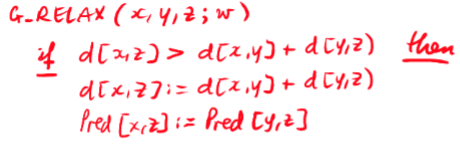
\includegraphics[width=0.4\linewidth]{Images/cammini_minimi/coppie/g_relax.png}
\end{figure}
Anche la funzione di inizializzazione diventa:
\begin{figure}[H]
    \centering
    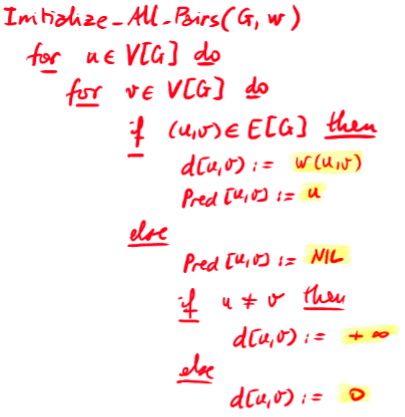
\includegraphics[width=0.3\linewidth]{Images/cammini_minimi/coppie/g_inizzializzazione.png}
\end{figure}

\subsection{Bellman-Ford per Coppie}
Una possibile soluzione si ottiene iterando l'algoritmo Bellman-Ford come segue:
\begin{figure}[H]
    \centering
    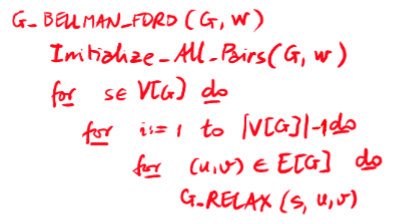
\includegraphics[width=0.3\linewidth]{Images/cammini_minimi/coppie/g_bellman_ford.png}
\end{figure}
Tale algoritmo ha complessità $O(V^2E)$ per grafi, cioè con $E=\Theta(V^2)$, tale complessità diventa $O(V^4)$.
Questo algoritmo non è molto efficiente nel costruire cammini lunghi. Immaginiamo questa situazione:
\[v_1 \to v_2 \to v_3 \dots \to v_7\]
Con l'approccio Bellman-ford abbiamo bisogno di calcolare prima $g\_relax(v_1,v_2,v_3)$, poi $g\_relax(v_1,v_3,v_4)$, poi $g\_relax(v_1,v_4,v_5)$, poi $g\_relax(v_1,v_5,v_6)$ e, infine, $g\_relax(v_1,v_6,v_7)$. Ma tante altre combinazioni di g\_relax sono possibili. Esiste un modo per ridurre il numero di chiamate $g\_relax$?

\subsection{Algoritmo Floyd-Warshall}
L’algoritmo in questione, si focalizza sui \textbf{vertici intermedi} di un cammino minimo che 
sarebbero i vertici che sono tra il vertice sorgente e quello di arrivo. Su un cammino semplice $p = (v_0,\dots, v_l)$ i vertici intermedi sono $(v_1, \dots, v_{l-1})$.
Organizzeremo il lavoro in "blocchi" che chiameremo $y_i$ e, in sostanza, quello che faremo a ogni iterazione è controllare se passare dal blocco $y_i$ aiuta ad arrivare a destinazione. L'idea è che se seguiremo un ordine qualunque di rilassamento di questi blocchi, otterremo quello che ci serve poiché:
\begin{itemize}
    \item Al passo $k$, calcoliamo i cammini minimi tra tutte le coppie $(i, j)$ potendo usare come nodi intermedi (ponti) solo i nodi che appartengono all'insieme $\{y_1, y_2, \dots, y_k\}$.
    \item Al passo $k+1$, aggiungiamo il nodo $y_{k+1}$ all'insieme dei nodi intermedi utilizzabili e vediamo se questo nuovo "ponte" ci permette di accorciare qualche percorso.
\end{itemize}
Alla fine di questa procedura avremo considerato tutti i nodi come intermediari piuttosto che andare a confrontare tutti i nodi come a casaccio e non è necessario che li analizziamo secondo un particolare ordine. 

\begin{figure}[H]
    \centering
    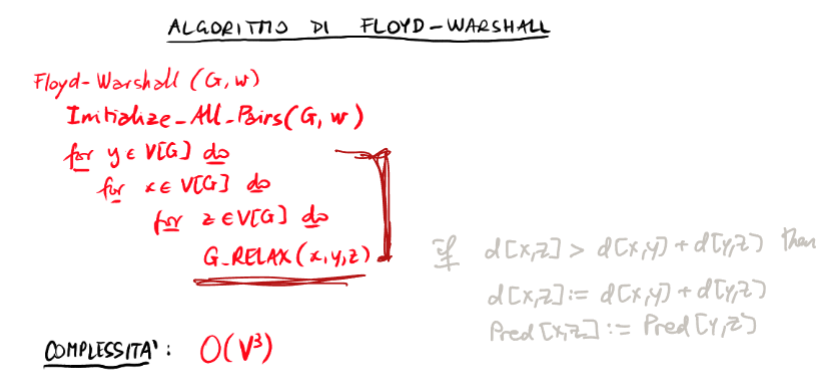
\includegraphics[width=0.6\linewidth]{Images/cammini_minimi/coppie/floyd_warshall.png}
\end{figure}

Dimostriamo che questo algoritmo funziona.  Sia $v_1,\dots, v_n$ l'ordine in cui gli elementi $y \in V$ vengono processati nel ciclo for più esterno. Per $1 \leq i \leq n$ e $u,v \in V$ poniamo $\delta^i(u,v)$ come il peso di un cammino semplice da u a v i cui nodi interni sono $\{v_1, \dots, v_i\}$. Possiamo dimostrare per induzione che dopo l'i-esima prova del ciclo for più esterno valgono:
\begin{itemize}
    \item $d[u,v]$ peso di un cammino $\pi$ da u a v i cui nodi interni sono in $\{v_1, \dots, v_i\}$ e, tale che $w(\pi) \leq \delta^i(u,v)$.
    \item $pred[u,v]$ predecessore di v in un cammino $\pi$ da u a v i cui nodi interni sono in $\{v_1, \dots, v_i\}$ e, tale che $w(\pi) = d[u,v]$
\end{itemize}
Per tanto, se il grafo iniziale ammette cammini minimi, allora varrà che:
\begin{itemize}
    \item $d[u,v] = \delta_{G,w}(u,v)$ per ogni coppia $u,v$
    \item $pred[u,v]$ predecessore di v in un cammino semplice da u a v. 
\end{itemize}
In sostanza, avremo che $d[u,u]= 0$ per ogni nodo e un cammino da u a v sarà dato dalla successione di predecessori di $v$. Esiste questo algoritmo per trovare il cammino:
\begin{figure}[H]
    \centering
    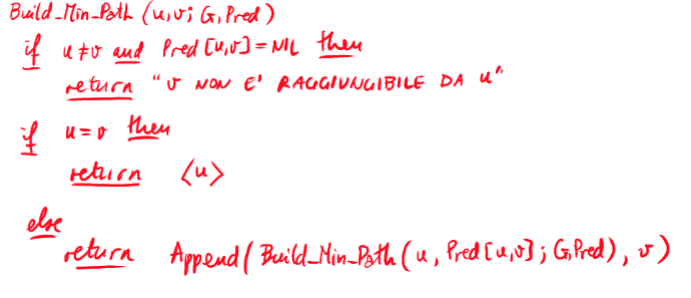
\includegraphics[width=0.6\linewidth]{Images/cammini_minimi/coppie/build_cammino.png}
\end{figure}
Nel caso in cui il grafo non ammette cammini minimi, alla fine dell'esecuzione di floyd warshall si ha che:
\[d[u,v]\leq \delta^n (v,v) \leq w(\pi)<0\]
Cioè avremo una condizione \textbf{necessaria e sufficiente perché ammetta cammini minimi} è che alla fine dell'esecuzione di floyd warshall si abbia che $d[u,u] = 0$ per ogni vertice. 

Immaginiamo di voler costruire un nuovo grafo $G^*$ (o una matrice) che ha un arco tra $u$ e $v$ se e solo se esiste un modo per raggiungere $v$ partendo da $u$ nel grafo originale. 
Per fare ciò, possiamo modificare la funzione peso in maniera tale che ogni arco abbia costo 1 e poi lanciando Floyd Warshall notiamo che se v è raggiungibile da u, allora $d[u,v] \neq \inf$ altrimenti sarà $\inf$. Esiste una versione ottimizzata di Floyd Warshall per fare questa cosa che sfrutta gli and e gli or logici per ottimizzare il tempo di calcolo sulla CPU.

\section{Rompere la barriera $O(V^3)$}
Con l'algoritmo Floyd Warshall arriviamo a una complessità di $O(V^3)$ e adesso ci domandiamo, possiamo fare di meglio? 

Nel caso in cui non vi siano archi di peso negativo, possiamo utilizzare Dijkstra $V$ volte che, implementandolo con gli \textbf{Heap di Fibonacci}  ha complessità di $O(V \log V + E)$ e, quindi, per $V$ iterazione abbiamo un costo totale di $O(V^2 \log V + VE)$. 
Il nostro nuovo algoritmo è asintoticamente migliore di $V^3$ se e solo se il grafo è sparso $E = o(V^2)$
\[V^2\log V + VE = o(V^3)\]
Poiché:
\begin{figure}[H]
    \centering
    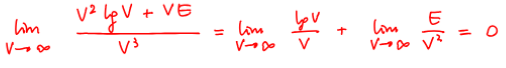
\includegraphics[width=0.5\linewidth]{Images/cammini_minimi/coppie/dimostrazione_multiple_dij.png}
\end{figure}

\subsection{Algoritmo di Johnson per Grafi Sparsi}
Questo algoritmo funziona anche con archi di peso negativo e sfrutta Dijkstra e Bellman-Ford come subroutines per ottenere una complessità di $O(V^2 \log V +VE)$.
Per fare ciò, l'algoritmo usa la tecnica del \textbf{riassegnamento dei pesi} $w \to \hat{w}$. Poiché Dijkstra si "rompe" se vede numeri negativi, Johnson trasforma il grafo originale $(G, w)$ in un nuovo grafo $(G, \hat{w})$ dove tutti i pesi sono non-negativi ($\hat{w} \ge 0$). È necessario che questa modifica venga effettuata in maniera tale che per ogni coppia $(u,v)$ il cammino $\pi_{uv}$ sia minimo in entrambi.\\
\textbf{Lemma:}\\
Sia $G=(V,E)$ un grafo con funzione peso $w: E \to R$ e sia $h:V \to R$ una funzione qualunque, si ponga:
\[\hat{w}(u,v) = w(u,v)+h(u)-h(v)\]
Per ogni $(u,v)\in E$. Allora per ogni cammino in G avremo che $\pi$ è un cammino minimo in $(G,w)$ se e solo se $\pi$ è un cammino minimo in $(G,\hat{w})$. Inoltre, $(G,w)$ ammette cammini minimi se e solo se $(G,\hat{w})$ li ammette.\\
\textbf{Dimostrazione:}\\
Sia $\pi = (v_0, \dots, v_k)$ un cammino in G, allora:
\[\hat{w}(\pi) = w(\pi)+h(v_0)-h(v_k)\]
Questo deriva da:
\begin{figure}[H]
    \centering
    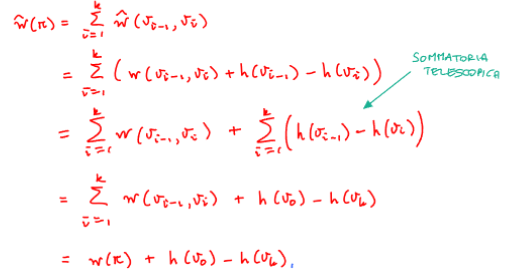
\includegraphics[width=0.6\linewidth]{Images/cammini_minimi/coppie/dimostrazione_john.png}
\end{figure}
Dato che $h(\text{Partenza})$ e $h(\text{Arrivo})$ sono costanti fisse per quel viaggio, se il cammino A era più breve del cammino B nel vecchio sistema, lo sarà anche nel nuovo.

Sia $\pi$ un cammino minimo in $(G,\hat{w})$ da u a v. Se $\pi$ non fosse minimo in $(G,w)$, allora esisterebbe un cammino $\pi'$ da u a v tale che $w(\pi')< w(\pi)$ ma \[\hat{w} = w(\pi') + h(u)-h(v) < w(\pi) + h(u) - h(v) = \hat{w}(\pi)\]
Contraddicendo la minimalità di $\pi$ in $(G,\hat{w})$, pertanto $\pi$ è minimo in $(G,w)$. Allo stesso modo, se $\pi$ è minimo in $(G,w)$ lo sarà anche in $(G,\hat{w})$. Inoltre, se $\pi= (v_0, v_k)$ è un ciclo con $v_0 = v_k$, allora $\hat{\pi} = w(\pi) + h(v_0) - h(v_k) = w(\pi)$. Di conseguenza, $(G,w)$ ammette cicli se e solo se li ammette anche $(G,\hat{w})$.\\
Vediamo adesso \textbf{come scegliere $h:V \to R$}. Vogliamo che i nuovi pesi siano tutti non negativi ($\hat{w} \ge 0$) per poter usare Dijkstra. Dalla formula vista prima, questo significa:
\[w(u,v) + h(u) - h(v) \ge 0 \quad \Rightarrow \quad h(v) - h(u) \le w(u,v)\]
Estendiamo, dunque, G con un nuovo nodo s e con archi $(s,v)$ per ogni $v \in V$ con $w(s,v) = 0$. Supponiamo che $(G',w)$ ammetta cammini minimi da s, si ponga $h(v) = \delta_{(G',w)}(s,v)$\footnote{Questo valore sarà procurato dall'algoritmo di Bellman-Ford. Probabilmente, la distanza minima $\delta$ sarà negativa a causa degli archi di peso negativo.} per ogni $v \in V$. Allora, per ogni arco $(u,v) \in E$ se $\pi_{su}$ è un cammino minimo da s a u si ha che: 
\begin{figure}[H]
    \centering
    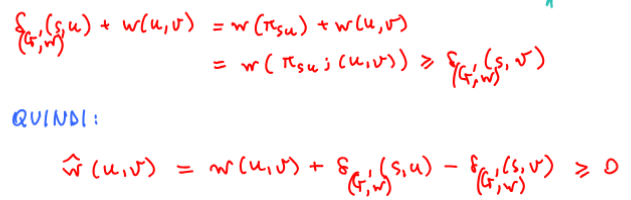
\includegraphics[width=0.6\linewidth]{Images/cammini_minimi/coppie/dim_john.png}
\end{figure}
Vediamo adesso il codice:
\begin{figure}[H]
    \centering
    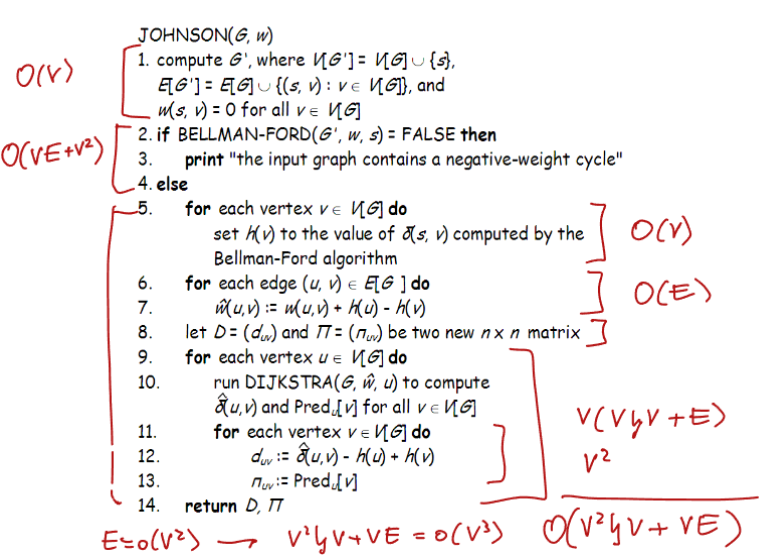
\includegraphics[width=0.8\linewidth]{Images/cammini_minimi/coppie/codice_john.png}
\end{figure}